\documentclass[a4paper]{IEEEtran}

\usepackage{graphicx}
\usepackage{hyperref}
\usepackage{tabularx}
\usepackage{multirow}
\usepackage{tikz}
\usepackage{pgfplots}

\usepgfplotslibrary{statistics}

\newcommand{\specialcell}[2][c]{%
\begin{tabular}[#1]{@{}c@{}}#2\end{tabular}}

\graphicspath{{illustrations/}}
\pgfplotsset{compat=1.8}

\pgfplotsset{
  /pgfplots/ybar legend/.style={
  /pgfplots/legend image code/.code={%
    \draw[##1,/tikz/.cd,yshift=-0.30em]
      (0cm,0cm) rectangle (3pt,0.8em);},
  },
}

\begin{document}

\setlength{\tabcolsep}{10pt}
\renewcommand{\arraystretch}{1.25}

\begin{center}
  \textbf{\Large{
    Imagely: A cloud environment for online image processing
  }}\\
  \vspace{0.25cm}
  \emph{Authors}: SB~Ramalingam Santhanakrishnan (4740270), \\ K~Kleeberger (4748476) and B~Jain (4745507)\\
  ICT Innovation, EEMCS, TU Delft\\
  \emph{Emails}: \{S.B.RamalingamSanthanakrishnan, K.Kleeberger, B.Jain\}@student.tudelft.nl\\
  \vspace{0.2cm}
  \emph{Course Instructors}: DHJ~Epema, A~Iosup and A~Kuzmanovska\\
  PDS Group, EEMCS, TU Delft\\
  \emph{Emails}: \{D.H.J.Epema, A.Iosup, A.Kuzmanovska\}@tudelft.nl\\
  \vspace{0.2cm}
  \emph{Lab Assistant}: BI~Ghit\\
  PDS Group, EEMCS, TU Delft\\
  \emph{Email}: B.I.Ghit@tudelft.nl\\
  \vspace{0.2cm}
  \emph{Teaching Assistant}: A~Parthasarathy\\
  EEMCS, TU Delft\\
  \emph{Email}: A.Parthasarathy@student.tudelft.nl\\
\end{center}

\vspace{0.2cm}

\textbf{
  \emph{Abstract}---\emph{Imagely} is a cloud service for batch image processing, designed for the specific requirements of WantCloud BV. Images are submitted by the end user, which are then processed by the service and the user is notified. It runs on Amazon Web Services (AWS) IaaS barebone compute resources to provide elastic scaling capabilities and its system design adapts the standard master-worker batch processing reference architecture pattern provided by AWS. The scheduler and provisioner are written in NodeJS in reactive style. We run three workloads each on three combinations of VM and scheduling policies with a hundred images. We show that the system
  can stay responsive under peak load to more than 50\% of the traffic at under 40 seconds while reducing the overall workload completion time. 
}

\section{Introduction}

WantCloud BV is a popular image processing company and are pioneers in converting raw satellite images to standard image formats consumable by users on the web browser. As the company is expanding into other domains and 
adding new customers rapidly, their existing deployment is unable to cope up with peak traffic demands and
 maintain service level agreements (SLAs). Thus, WantCloud BV is evaluating an IaaS-based solution that
 can scale with the demand.

The proposed system utilizes Amazon Web Services (AWS)~\cite{aws} IaaS cloud service provider's compute instance, EC2 (Elastic Cloud Compute) for providing on-demand compute capacity to process the workloads.
We design a custom provisioner and scheduler using the AWS low-level SDK, EC2 API for requesting and releasing virtual machine instances (VMs).
We also utilize Amazon Machine Images (AMIs) for pre-packaging the application code,
configuration information and the operating system for the instance to save time during its launch. For image processing and conversion, we use the ImageMagick~\cite{imagemagick} program. We wrap ImageMagick with a thin HTTP server written in NodeJS~\cite{nodejs}, which forks ImageMagick as a child process and performs read/write through stdin/stdout pipes, the instances which perform image processing are known as
the workers. For analysis purposes, we restrict the scope of the worker to scaling down, rotating and converting the
image from TIFF~\cite{rfc3302} to JPEG format~\cite{jpeg}.

The system design follows the AWS reference architecture for batch processing~\cite{aws_batch}, we differ in that we have
implemented our own custom scheduler and provisioner in a reactive fashion and have placed all the task queues and resource management responsibilities on the master node. The master node accepts the image processing task requests via HTTP and launches multiple worker nodes, based on the given policy. It then balances and allocates the tasks to the workers and also monitors the progress. It also keeps accumulating reports on completion of each task and launch/release of each instance during its lifetime. The policy targets the provisioner with parameters for minimum and maximum
number of workers to launch and the scaling-up decision threshold.

The test workload is a collection of 100 TIFF images from NASA's publicly available Landsat satellite image repository \cite{landsat_s3}, file sizes ranging from 40-60 MB. To determine the baseline (current) effort required, we run the workload on a static VM deployment and to analyse the scaling and scheduling capability of the cloud solution, we test the workload with two well-known policies. The workload itself is varied with three exponential Poisson~\cite{jain1990art} mean arrival time distributions to simulate realistic traffic patterns.

In \autoref{application}, additional background information on the application is provided. In \autoref{system_design} we illustrate the design of the system in detail with focus on specific aspects pertaining to
WantCloud's requirements and in \autoref{experiments} we present the experiments conducted along with the
results and analysis. We conclude the report in \autoref{conclusion} with a short discussion on the findings and potential improvements.

\section{Application} \label{application}

The web-based application receives tasks from end-users in JSON format~\cite{rfc7159}, which point to a source image URL and defines a sequence of image manipulation operations such as scaling, rotation and finally file format conversion from TIFF to JPEG. This JSON request is forwarded to an idle worker in the resource pool by the master node. Internally, ImageMagick program is used for processing the image and it is forked by the worker's NodeJS web server. The application is I/O bound during retrieval of the source image and writing the result to AWS S3 storage (the NodeJS web server handles all I/O), CPU and memory intensive when it performs the actual image manipulation and conversion. A task is declared to be a failed if any of the above three steps encounter an error or the entire task does not complete within 30 seconds.

\subsection{Requirements}

In order to replace WantCloud's current system, the following requirements are to be met by the new system.

\begin{itemize}
  \item \emph{Automation}: The system should be automated for creation, provisioning and other activities
  with minimal human intervention.
  \item \emph{Auto-scaling}: The system should be able to detect fluctuations in demand and scale up or down the VM resource pool automatically.
  \item \emph{Load Balancing}: The system should be able to best utilize the available pool of compute resources
  for the workload through allocation policies.
  \item \emph{Reliability}: The system should be able to retry failed tasks, ensure availability through redundancy and recover from unexpected failures.
  \item \emph{Monitoring}: The system should be able to keep track of resource usage and provide information
  on metrics to aid future decisions.
\end{itemize}

\begin{figure}[tbp]
  \centering
    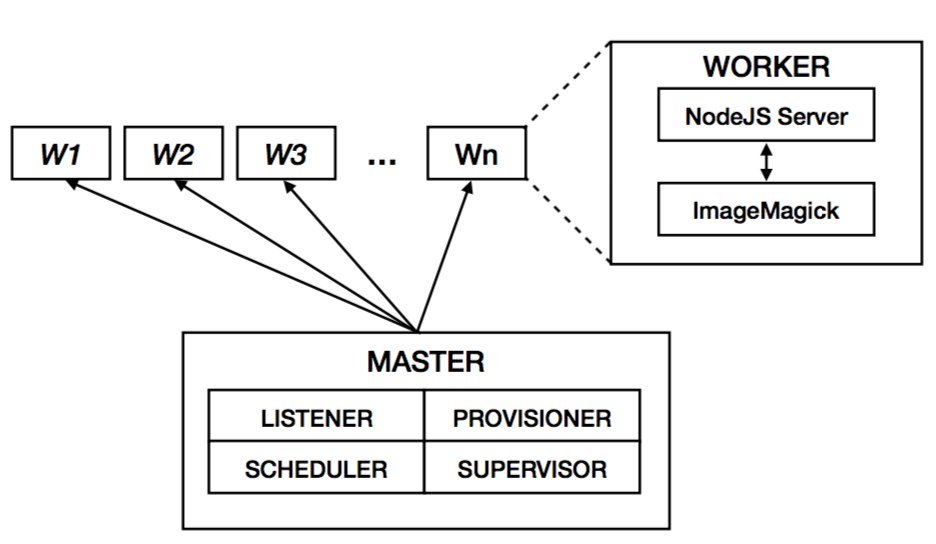
\includegraphics[width=\columnwidth]{system-design.png}
  \caption{Overview of system design.}
  \label{fig:overview_system_design}
\end{figure}

\section{System Design} \label{system_design}

As mentioned in \autoref{application}, the server (master node) accepts the tasks and adds it to the pending task queue. The task is then allocated by the scheduler to an available worker instance at the next scheduling cycle. The workers finish the task and notify the end-user via E-mail about the job completion or failure, the stored location of the result and returns control to the master with usage info.

\subsection{Overview} \label{system_design_overview}

The system, illustrated in \autoref{fig:overview_system_design} consists of the following components, placed in the master node:

 \begin{itemize}
   \item \emph{Listener}: The NodeJS server, which accepts client requests through HTTP, parses it, creates a 
   corresponding internal task representation and adds it to the pending task queue.
   \item \emph{Scheduler}: The scheduler is invoked as soon as a task enters the pending queue (debounced by 1 second) or it is invoked by the system periodically. It matches tasks in the pending queue to free worker instances in the resource pool.
   \item \emph{Provisioner}: The provisioner manages the request and release of worker instances in the resource 
   pool according to the given policy.
   \item \emph{Supervisor}: The supervisor is responsible for bootstrapping the system, monitoring the finished/failed tasks, monitoring health of the instances, maintaining an audit log of all the tasks and instances to generate a report when requested and finally perform cleanup and release of instances on unexpected shutdown (SIGINT, SIGTERM)
   if possible\footnote{During bootstrap, it queries AWS for any existing workers and adds them to the resource pool.}.
 \end{itemize}

\subsection{Resource Management Architecture}
 
\begin{figure}[bp]
  \centering
    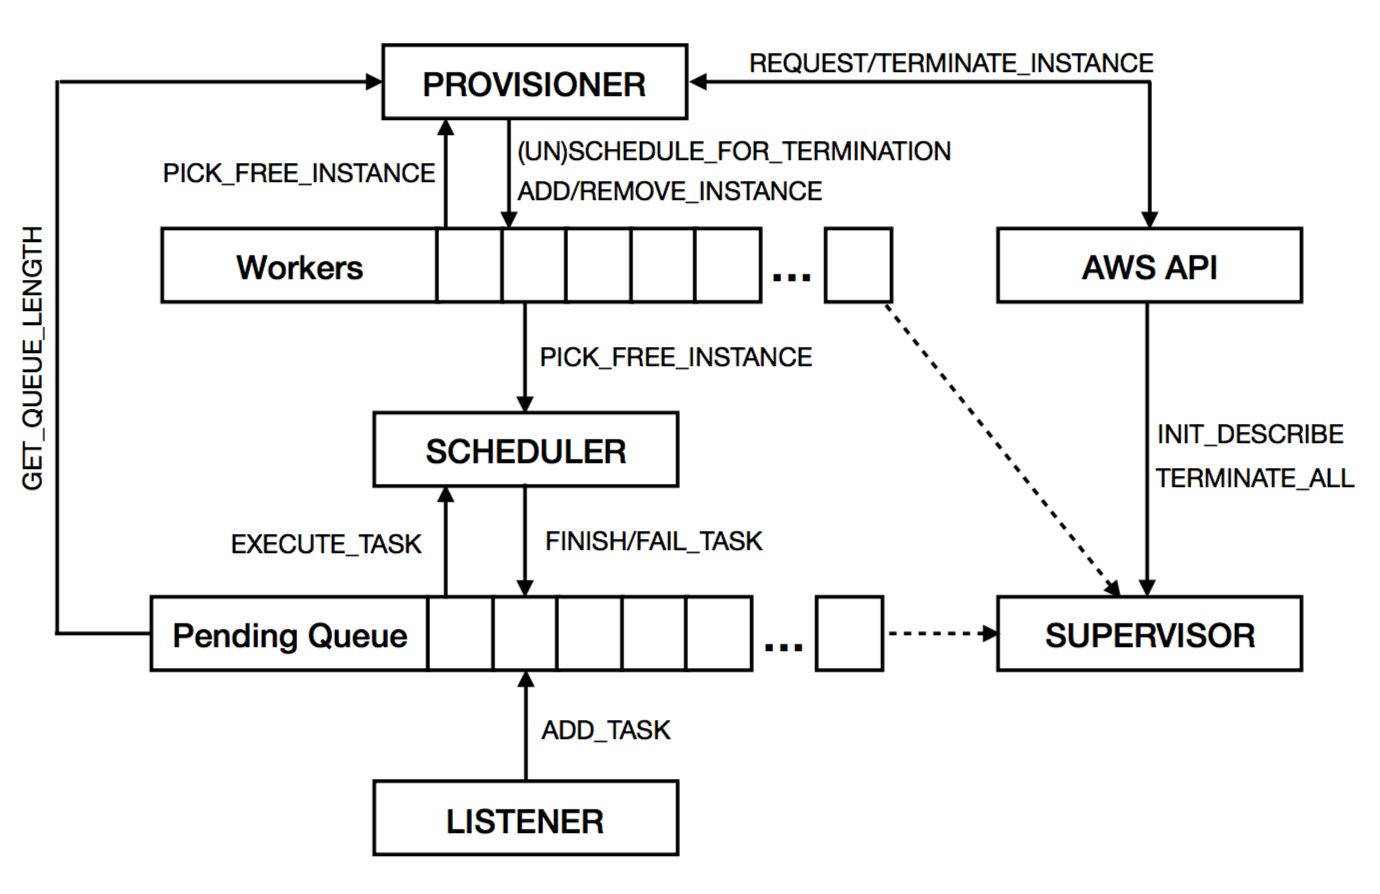
\includegraphics[width=\columnwidth]{resource-management.png}
  \caption{Resource management architecture with message flows.}
  \label{fig:resource_management}
\end{figure}

The components listed in \autoref{system_design_overview} each have their own life cycle and associated events.
Since we follow the reactive pattern, we illustrate the resource management architecture by tracing the execution
 of a task through the system, handled by the various components across phases listed below and in \autoref{fig:resource_management}.

\begin{enumerate}
  \item \emph{Bootstrap}: This phase marks the start of the system, before the arrival of tasks. The supervisor starts the scheduler, provisioner and the listener and 
  broadcasts a \textsc{Bootstrap} event which the components listen to and perform initial setup activities if any. The supervisor
  also invokes the AWS API with a \textsc{Describe} call to get a list of already started workers if any, this is essential to prevent
  orphaned nodes in case the master restarts from a failure recovery.

  \item \emph{Scheduling and Allocation}: The listener listens for incoming tasks from end-users and adds it to the pending queue
  with the \textsc{Add\_Task} event, after marking the arrival time. The scheduler picks
  tasks from the pending queue, picks free instances from the worker pool, matches the two and publishes the \textsc{Execute\_Task} event.
  Another part of the scheduler asynchronously listens to \textsc{Execute\_Task}, invokes the worker node, waits till 
  the task is finished/failed and adds it to the pending queue again on failure. The allocation of jobs to workers
  is influenced by three policies -- priority of tasks in the pending queue, criteria of allocation to a worker instance and
  the maximum number of retries for a failed task.

  \item \emph{Provisioning}: The provisioner is also invoked periodically and performs two duties -- pick free instances from the 
  resource pool for termination, request for a new instance based on the given policy. As soon as we request the AWS API
  for a new instance, we repeatedly hit the health check HTTP endpoint of the worker application to determine if it is ready\footnote{This is possible in AWS because EC2 allocates a private IP address to the instance as soon as the request is made. In case this 
  is not possible with the cloud provider, we additionally wait for the IP address to be allocated before beginning health checks.}.
  If it is ready before a timeout, it is added to the worker pool else terminated immediately. Note that in regular cases we do not terminate immediately,
  instead we first schedule a worker for termination in the future with \textsc{Schedule\_For\_Termination} event, to prevent thrashing.
  A separate part of the scheduler listens to this event, waits for the scheduled time and then releases instance by calling AWS API, however during the
  wait, it also intercepts any calls to request for new instance, cancels the termination schedule and adds the instance back to the pool.
  The policies applied to provisioning are the minimum/maximum number of instances to maintain, queue threshold for scaling
  decisions, and the worker instance type to launch.

  \item \emph{Termination and Reliability}: During the termination phase, the supervisor shuts down each instance in
  the resource pool with a \textsc{Terminate\_All} call. The reliability of the system is ensured by configuring auto-restart
  of the master process in the host operating system and running it as a daemon process. The supervisor also maintains
  an audit trail of the system, which can be retrieved via an HTTP endpoint for inspection. Since the system is
  single threaded we make sure that the queue and resource pool data structures are maintained in a single
  immutable store and updated only via invocation of events.
  
  To determine the health of the instances, when a task fails, the supervisor runs a health check on the instance
  on which the task failed. The failure of the health check leads to immediate termination of the instance.

\end{enumerate}

\subsection{System Policies}

In the system, we have implemented one scheduling policy and one allocation policy illustrated below.

\begin{enumerate}
  \item \emph{Scheduling}: The scheduler implements the first come, first serve (FCFS) policy.
  It picks the task with the earliest arrival time and maximum retry count for execution on the next available worker instance.

  \item \emph{Provisioning}: We implement \textsc{On-Demand Single VM (OD-S)} policy~\cite{villegas2012analysis}, which allocates 
  one VM per job and releases the VM after job completion plus a wait time (10 seconds in our case). The decision on provisioning
  of new instances is taken when the pending task queue length goes above the given threshold.

  The configurable parameters of the OD-S policy are,
    \begin{itemize}
      \item \emph{min-vms}: The minimum number of VMs the system must have at any point.
      \item \emph{max-vms}: The total number of VMs the system can provision at most.
      \item \emph{threshold}: The pending queue length at which the provisioner is allowed to start a new instance. 
    \end{itemize} 

  \item \emph{Progress Condition}: The system however ensures that a minimum of 1 instance is running in case there are 
  tasks in the pending queue irrespective of the threshold policy. 

  \item \emph{Termination}: When the pending queue length falls below the threshold, the scheduler marks instances to be
  terminated and the provisioner executes the termination after the wait period.
\end{enumerate}

The components of the system intercept events and lookup the central immutable store in order to enforce the policies. 
This flexibility enables us to implement various other policies by consuming the entire state of the 
system at any point in time. The system parameters are summarized in \autoref{table:system_params}, * indicates that we have varied the value according to experiments in the following section.

\begin{table}[tbp]
  \centering
  \caption{System parameters and values in implementation.}
  \label{table:system_params}
  \begin{tabular}{|r|r|}
    \hline
     MAX\_RETRIES & 5 \\
     MIN\_VMS & * \\
     MAX\_VMS & * \\
     THRESHOLD & * \\
     MAX\_RETRIES & 5 \\
     SCHEDULER\_INTERVAL & 5s \\
     TASK\_TIMEOUT & 25s \\
     PROVISIONER\_INTERVAL & 5s \\
     HEALTH\_CHECK\_INTERVAL & 1s \\
     INSTANCE\_READY\_TIMEOUT & 60s \\
     TERMINATION\_WAIT\_TIME & 10s \\
     \hline
  \end{tabular}
\end{table}

\section{Experimental Results} \label{experiments}

We conduct a total of 9 experiments and analyse the results in the following sub-sections.

\subsection{Setup}

The goal of the experiments is to analyse the tradeoffs between WantCloud BV's current 
system (3 dedicated servers) versus the proposed IaaS cloud based solution by estimating the workload
processing time, responsiveness and the cost. The key components of the system under test are the scheduler
and provisioner, affected by the factors, task arrival time and threshold for scaling.

The test system is deployed on the AWS cloud platform using bare bone EC2 compute instances. We
use the m3.medium type (vcpus=1, memory=3.75Gb based on Intel Xeon E5-2670 v2) for both the master and the worker. 
We restricted the deployment to a single region, North Virginia (US-East-1) with default availability zone placement policy and the default 
virtual private cloud settings provided by AWS. A custom security group is used for exposing ports 8000 (master),
 3000 (worker) and 3001 (worker health check) for inbound TCP (HTTP) traffic, the worker nodes however do not 
 have public IP address and are reachable only by the master via HTTP.

 The workload consists of 100 images from the Landsat satellite in TIFF format and each task consists of
 scaling the image size down to a factor of 0.25, rotation by 90 degrees clockwise and finally conversion to 
 TIFF format. We have three sets of 100 requests by varying the inter-arrival time through Poisson distribution
 with mean intervals of 2.5, 5 and 7.5 seconds labelled as \textsc{W(2.5)}, \textsc{W(5)} and \textsc{W(7.5)}. The
 system has been written in Typescript~\cite{typescript}, targeting NodeJS version 8 using ReactiveX extensions~\cite{reactivex}. The express~\cite{express} framework has
 been used for the web server and ElasticSearch~\cite{elasticsearch} has been used for analysing time series results obtained from the audit log report. 

\subsection{Experiments}

We run the workload on three variations of system policies by adjusting the parameters,
 firstly \textsc{C3} -- constantly 3 VMs, which represents the current setup of WantCloud BV, secondly \textsc{E0} -- elastic 0-15 VMs with threshold set to 0 and thirdly, \textsc{E7} -- elastic 0-15 VMs with threshold set to 7. The factors target the load balancing and provisioning policy of the system. In the following sections we present the analysis.

\subsubsection{Overheads}

The average VM allocation overhead by AWS was found to be 42 seconds and we did not find any significant network overheads. However, to prevent any disruptions due to network, we placed a workload driver instance in the same availability zone subnet as of the master node and ran the experiments.

\subsubsection{Processing time}

The total time the system took to process the entire workload, presented
in \autoref{fig:processing_time}, shows that E0 takes the least amount of time (272 seconds) for W(2.5). However, E0 performs the worst as the mean arrival time starts to increase. This can be directly attributed to the fact that the policy is very aggressive in releasing VMs and thus a lot of thrashing is experienced.

\begin{figure}[bp]
  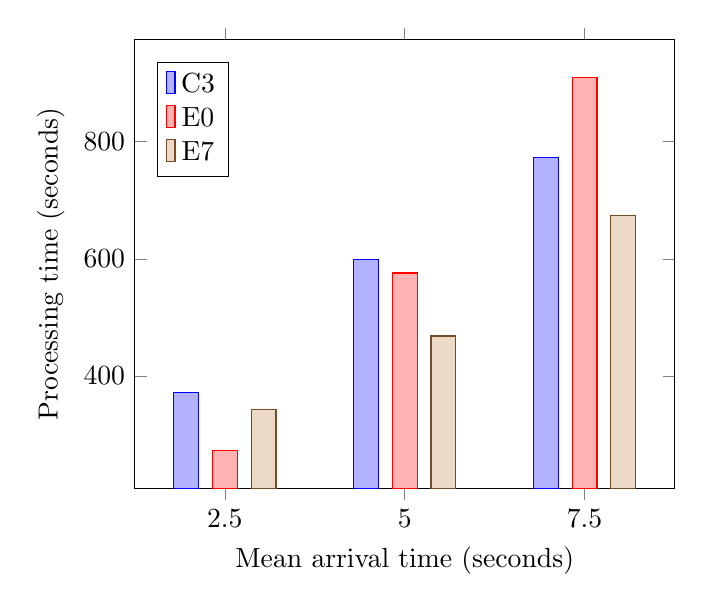
\begin{tikzpicture}
    \begin{axis}[
      xtick=data,
      ylabel = Processing time (seconds),
      xlabel = Mean arrival time (seconds),
      legend style={at={(0.175, 0.95)}},
      enlarge x limits=0.25,
      ybar=5pt,
      bar width=9pt,
    ]
    \legend{C3, E0, E7}
    \addplot coordinates {
      (2.5, 372.347) (5.0, 599.254) (7.5, 772.459)
    };
    \addplot coordinates {
      (2.5, 272.241) (5.0, 575.742) (7.5, 910.306)
    };
    \addplot coordinates {
      (2.5, 343.241) (5.0, 468.092) (7.5, 673.886)
    };
    \end{axis}
  \end{tikzpicture}
  \caption{Workload processing time across three mean arrival times.}
  \label{fig:processing_time}
\end{figure}

\subsubsection{Responsiveness}

The metric for responsiveness is derived from the average waiting time of the tasks in the pending queue until they are scheduled for execution, presented in \autoref{fig:waiting_time}. Contrary to our expectations, we see that \textsc{C3} has the least average wait time of 7.5 seconds at 595.6 seconds for W(7.5). We also observe that \textsc{E0} maintains 
a consistent wait time for both W(5) and W(7.5). However, on closer inspection, we found that the  waiting time average has been heavily skewed by a few outliers affected by the provisioner. We focus
on the results of W(2.5) in \autoref{fig:response_time_box_plot}, where majority of the tasks for
E0 and E7 lie below 40 seconds. This large waiting time occurs for a few tasks when a free VM is not found and the provisioner is still starting a new instance, causing all the tasks in the queue to starve. This happens when the system starts the first instance (correlates to $\approx$40 seconds instance startup overhead) and also in one another case when all the VMs are shut down to 0. 

We also found task retries to be playing a role here. The failed task enters the pending queue with highest priority and also the instance on which the task failed is now marked for health check, effectively taking away one worker from the pool for a few seconds. This specific case occurred in E7 when there was only 1 instance running, a task failed and there were 5 other tasks (7 is threshold) in the pending queue.

\begin{figure}[tbp]
  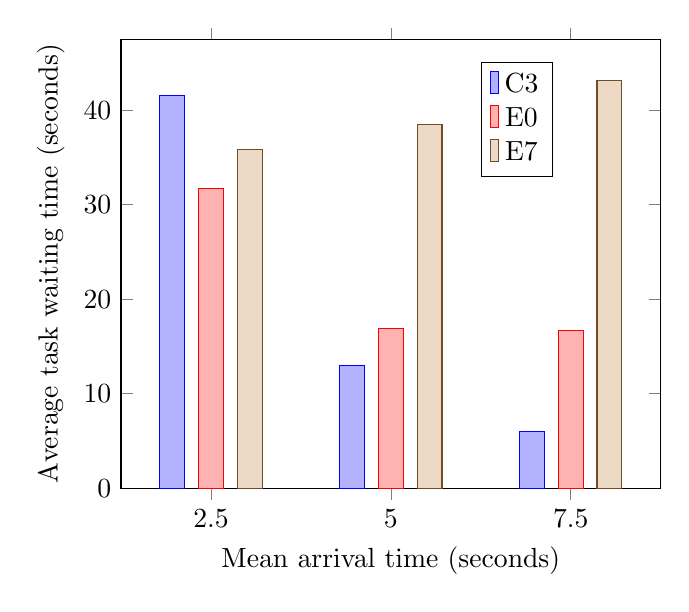
\begin{tikzpicture}
    \begin{axis}[
      xtick=data,
      ylabel = Average task waiting time (seconds),
      xlabel = Mean arrival time (seconds),
      legend style={at={(0.80, 0.95)}},
      enlarge x limits=0.25,
      ybar=5pt,
      bar width=9pt,
      ymin=0,
    ]
    \legend{C3, E0, E7}
    \addplot coordinates {
      (2.5, 41.55456) (5.0, 13.01204) (7.5, 5.956)
    };
    \addplot coordinates {
      (2.5, 31.72191) (5.0, 16.89337) (7.5, 16.66199)
    };
    \addplot coordinates {
      (2.5, 35.81022) (5.0, 38.47375) (7.5, 43.13281)
    };
    \end{axis}
  \end{tikzpicture}
  \caption{Cumulative task waiting time for workload across arrival times}
  \label{fig:waiting_time}
\end{figure}

\begin{figure}[tbp]
  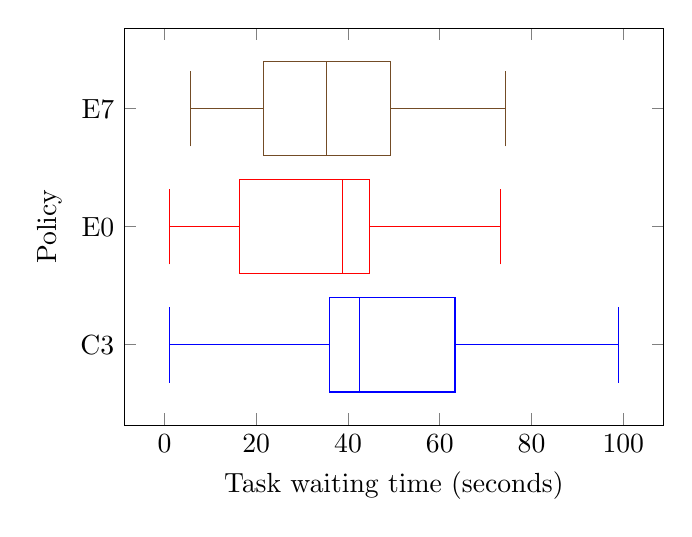
\begin{tikzpicture}
    \begin{axis}[
      boxplot,
      y=1.5cm,
      ytick={1, 2, 3},
      yticklabels={C3, E0, E7},
      ylabel = Policy,
      xlabel = Task waiting time (seconds),
    ]
    \addplot+ [boxplot prepared={
        lower whisker=1, lower quartile=35.979,
        median=42.439, upper quartile=63.313,
        upper whisker=99.012},
    ] coordinates {};
    \addplot+ [boxplot prepared={
        lower whisker=1, lower quartile=16.361,
        median=38.838, upper quartile=44.773,
        upper whisker=73.323},
    ] coordinates {};
    \addplot+ [boxplot prepared={
        lower whisker=5.668, lower quartile=21.489,
        median=35.396, upper quartile=49.284,
        upper whisker=74.232},
    ] coordinates {};
  \end{axis}
  \end{tikzpicture}
  \caption{Task waiting time distribution for W(2.5)}
  \label{fig:response_time_box_plot}
\end{figure}

\subsubsection{Utilization}

We analyse the utilization of the system presented in \autoref{fig:utilization} as the ratio of total VM time spent
in task execution to its total lifetime. The maximum utilization we see even for \textsc{C3} where there is no provisioning overhead is about 80\%. This highlights the drawback in the periodic invocation of the scheduler and provisioner. The VMs have to wait for the next scheduling/provisioning cycle until which they are going to be idle. Another cause is the scheduled termination time where the VM waits for 10 seconds before getting terminated. If a task arrives at its 8th second of wait time, the task will miss the VM anyway. 

This chart once again highlights the thrashing problem associated with \textsc{E0}, it is simply keeping around idle VMs due to termination wait time. However, we see a balanced utilization for \textsc{E7}, it gains from not letting the VM go away immediately as the allocation overhead is much larger and preventing VMs from having a short lifetime.

\begin{figure}[tbp]
  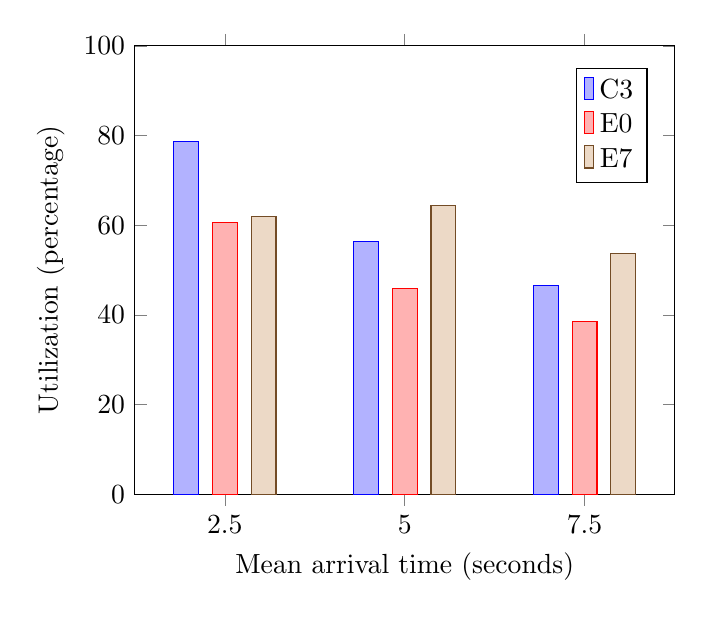
\begin{tikzpicture}
    \begin{axis}[
      xtick=data,
      ylabel = Utilization (percentage),
      xlabel = Mean arrival time (seconds),
      legend style={at={(0.95, 0.95)}},
      enlarge x limits=0.25,
      ybar=5pt,
      bar width=9pt,
      ymin=0,
      ymax=100,
    ]
    \legend{C3, E0, E7}
    \addplot coordinates {
      (2.5, 78.6) (5.0, 56.4) (7.5, 46.5)
    };
    \addplot coordinates {
      (2.5, 60.5) (5.0, 45.9) (7.5, 38.6)
    };
    \addplot coordinates {
      (2.5, 62.0) (5.0, 64.3) (7.5, 53.7)
    };
    \end{axis}
  \end{tikzpicture}
  \caption{Utilization of VMs for workload across arrival times}
  \label{fig:utilization}
\end{figure}

\subsubsection{Costs}

Each experiment (except C3 with constantly 3 workers) starts and stops several VMs over its processing time and our total instance run time is under 1 hour for each experiment. Therefore, the cost is computed in terms of hourly charges for unique instances launched, tabulated in \autoref{table:costs} for running m3.medium instance\footnote{In the real life however, AWS offers per second billing which would greatly reduce the cost, which our policies were designed for.}. Apart from the instance cost, there are minor acceptable costs involving the ephemeral disk storage, data transfer and AMI snapshots.

\begin{table}[hbp]
  \centering
  \caption{Charged cost per hour across arrival times}
  \label{table:costs}
  \begin{tabular}{|c|c|c|c|}
    \hline
    Policy & 2.5s & 5s & 7.5s \\
    \hline
    C3 & \$0.27 ~(4) & \$0.27 ~(4) & \$0.27 ~(4) \\
    E0 & \$1.88 (28) & \$3.89 (58) & \$6.16 (92) \\
    E7 & \$2.01 (30) & \$2.08 (31) & \$3.82 (57) \\
    \hline
  \end{tabular}
\end{table}

\subsection{Potential Improvements}

The experiments and analysis suggest that the \textsc{E7} policy is all round consistent with
all arrival times. We would like to improve in the following areas.

\begin{enumerate}
  \item Schedule more than one task in a worker, considering that 50\% of the time the worker is
  either downloading or uploading data.
  \item Scale up instances in multiples of 2 or geometrically.
  \item Run a worker process in the master node itself. This can further increase the responsiveness
  and save cost.
  \item Implement shortest job scheduling policy since the tasks can be roughly weighted with the input image size.
\end{enumerate}

Clearly there are many other drawbacks in our implementation which we wish to overcome. However the experiments gave deep insights into the various bottlenecks and optimization points in the system.

\section{Conclusion} \label{conclusion}

The speedups shown in \autoref{table:speedup} indicate that a maximum speedup of upto 1.38 times was achieve by our system. The chief requirement of WantCloud BV, is to maintain responsiveness at peak traffic demands, which is clearly met by the system, illustrated in \autoref{fig:response_time_box_plot}, where a majority of the traffic is scheduled for execution within 40 seconds, \textsc{W(2.5)}. The incidental costs of cloud when such a traffic is not present should also be noted though. However, the elastic policies can scale the system down to 0 workers, saving cost when there is no traffic. We found that in some cases it costs more than 10 times to finish the same amount of work with only a marginal speedup, indicating that policies must be chosen carefully. After analysing the tradeoffs, we think that it is cost-worthy for WantCloud BV to move their application to cloud.

\begin{table}[htbp]
  \centering
  \caption{Speedup}
  \label{table:speedup}
  \begin{tabular}{|c|c|c|c|c|}
    \hline
    \multirow{2}{*}{\specialcell{Arr.\\Time}} & \multicolumn{1}{|c|}{C3} & \multicolumn{1}{|c|}{E0} & \multicolumn{1}{|c|}{E7} \\
     & Speedup & Speedup & Speedup \\
    \hline
     W(2.5) & 1.0 & 1.38 & 1.09 \\
     W(5.0) & 1.0 & 1.04 & 1.28 \\
     W(7.5) & 1.0 & 0.84 & 1.14 \\
    \hline
  \end{tabular}
\end{table}

\bibliographystyle{myIEEEtran}
\bibliography{large-lab}

\section*{Appendix A: Time Sheets}

\begin{table}[htbp]
  \centering
  \caption{Time spent on the project per activity.}
  \begin{tabular}{| l | c |}
    \hline
    Activity & Time (hours) \\
    \hline
    Total & 170 \\
    Think & 20 \\
    Dev & 80 \\
    XP & 15 \\
    Analysis & 15 \\
    Write & 20 \\
    Wasted & 20 \\
    \hline
  \end{tabular}
\end{table}

\begin{table}[htbp]
  \centering
  \caption{Time spent per experiment.}
  \begin{tabular}{| l | r | r | r |}
    \hline
    & \multicolumn{3}{| c |}{Time (hours)} \\
    \hline
    & Dev & Setup & Total \\
    \hline
    C3 & 8 & 4 & 12 \\
    E0 & 1 & 0.5 & 1.5 \\
    E7 & 1 & 0.5 & 1.5 \\
    \hline
  \end{tabular}
\end{table}

\end{document}
